% THIS IS SIGPROC-SP.TEX - VERSION 3.1
% WORKS WITH V3.2SP OF ACM_PROC_ARTICLE-SP.CLS
% APRIL 2009
%
% It is an example file showing how to use the 'acm_proc_article-sp.cls' V3.2SP
% LaTeX2e document class file for Conference Proceedings submissions.
% ----------------------------------------------------------------------------------------------------------------
% This .tex file (and associated .cls V3.2SP) *DOES NOT* produce:
%       1) The Permission Statement
%       2) The Conference (location) Info information
%       3) The Copyright Line with ACM data
%       4) Page numbering
% ---------------------------------------------------------------------------------------------------------------
% It is an example which *does* use the .bib file (from which the .bbl file
% is produced).
% REMEMBER HOWEVER: After having produced the .bbl file,
% and prior to final submission,
% you need to 'insert'  your .bbl file into your source .tex file so as to provide
% ONE 'self-contained' source file.
%
% Questions regarding SIGS should be sent to
% Adrienne Griscti ---> griscti@acm.org
%
% Questions/suggestions regarding the guidelines, .tex and .cls files, etc. to
% Gerald Murray ---> murray@hq.acm.org
%
% For tracking purposes - this is V3.1SP - APRIL 2009

\documentclass{acm_proc_article-sp}
\usepackage{epstopdf}
%
%\usepackage[dvips]{graphicx}
\usepackage{epsfig}
%\usepackage[chapter]{theorems}
\usepackage{symbols}
\usepackage{url}
\usepackage{algorithm}
\usepackage{algorithmic}
\usepackage{color}
\usepackage{alltt}
\usepackage{dsfont}
\usepackage{upgreek}
\usepackage[tight]{shorttoc}
\usepackage{multirow}
\usepackage{rotating}
\usepackage{array}
\usepackage{colortbl}
\usepackage{xcolor}
\usepackage{listings}
\usepackage[rounded]{syntax}
\usepackage{slashbox}
\usepackage{graphicx, subfig}
\usepackage{enumerate}
\usepackage{amssymb}
\usepackage{appendix}
\usepackage{eurosym}
\usepackage{amsfonts}
\usepackage{pifont}
%\usepackage{hyperref}
\usepackage{pdflscape}
\usepackage{amsmath}
\usepackage{fixltx2e} 

\lstset{ %
        language=Prolog,                % the language of the code
        basicstyle=\scriptsize,       % the size of the fonts that are used for the code
        numbers=right,                   % where to put the line-numbers
        numberstyle=\scriptsize,      % the size of the fonts that are used for the line-numbers
        stepnumber=1,                   % the step between two line-numbers. If it's 1, each line 
                                % will be numbered
        numbersep=0.05cm,                  % how far the line-numbers are from the code
        backgroundcolor=\color{white},  % choose the background color. You must add \usepackage{color}
        showspaces=false,               % show spaces adding particular underscores
        showstringspaces=false,         % underline spaces within strings
        showtabs=false,                 % show tabs within strings adding particular underscores
        frame=none,                   % adds a frame around the code
        tabsize=3,                      % sets default tabsize to 2 spaces
        captionpos=b,                   % sets the caption-position to bottom
        breaklines=true,                % sets automatic line breaking
        breakatwhitespace=false,        % sets if automatic breaks should only happen at whitespace
        %title=\lstname,                 % show the filename of files included with \lstinputlisting;
                                   % also try caption instead of title
        escapeinside={\%*}{*)},         % if you want to add a comment within your code
        deletekeywords={not}
        %morekeywords={luents, actions, always, initial, if, inertial, after, inertial, noConcurrency,goal,not,caused,executable,nonexecutable,forbiden,requires}            % if you want to add more keywords to the set
}
\newcommand{\hlight}[2]{\begingroup \color{#1}#2 \endgroup}
\newcommand{\manolo}[2]{{\hlight{#1}{#2}}}

\def\ie{\textit{i.e.}}
\def\eg{\textit{e.g.}}
\def\cf{\textit{cf.}}
\def\aka{\textit{a.k.a.}}

\include{apis}
\newcommand\SeQLcode[3]{
	\lstinputlisting[language=SQL, morekeywords= {now, top}, caption={#1}, columns=fixed, label=#3]{#2}
}

\newcommand\PrologCode[3][]{
	\lstinputlisting[language=Prolog, morekeywords={fluents, actions, always, initial, if, inertial, after, inertial, noConcurrency,goal,not,caused,executable,nonexecutable,forbiden,requires}, caption={#1}, columns=fixed, label=#3]{#2}
}

\newcommand{\tickYes}{\checkmark}

\newcommand{\tickNo}{\hspace{1pt}\ding{55}}

\newcommand\dt[1]{$\mathtt{#1}$}

\newcommand{\sembrack}[1]{[\![#1]\!]}

\hyphenation{pro-du-cer ca-ta-log coor-di-na-tes de-pen-dent ge-ne-ra-tion pa-ra-lle-li-za-tion con-ti-nuous im-ple-men-ting exe-cu-tion apli-ca-tion acce-ssing answer know-ledge po-ssi-ble gene-rated abs-trac-tion diffe-rent}
\newcommand\tabsize[2]{
\begin{table}
   \begin{center}
       {\small
      \begin{tabular}{m{0.6cm} |m{1.4cm} m{1.4cm} m{1.4cm} m{1.4cm} }
  
         \hline
          \multirow{2}{*}{$l$}& \multicolumn{4}{c}{Workflows}\\
            & \textbf{W1} & \textbf{W2} & \textbf{W3} & \textbf{W4} \\
         \hline
         \hline
6 & 0 & 0 & 0 & 0 \\
7 & 4 & 4 & 20 & 20 \\
8 & 62 & 128 & 598 & 1192 \\
9 & 278 & 956 & 5062 & 15820 \\
10 & 578 & 3068 & 19822 & 90100 \\
11 & 718 & 5368 & 43698 & 277800 \\
12 & 718 & 6268 & 62358 & 525476 \\
13 & 718 & 6268 & 62358 & 749840 \\
14 & 718 & 6268 & 62358 & 749840 \\
         \hline     
      \end{tabular}
   }  
      \caption{#2}\label{#1}
      
     \end{center}
   \end{table}  
}

\newcommand\tabtime[2]{
\begin{table}
   \begin{center}
      \begin{tabular}{m{0.6cm} |m{1.4cm} m{1.4cm} m{1.4cm} m{1.4cm}}
         \hline
          \multirow{2}{*}{$l$}& \multicolumn{4}{c}{Workflows}\\
                              & \textbf{W1} & \textbf{W2} & \textbf{W3} & \textbf{W4} \\
         \hline
         \hline
 6&  0,00 & 0,00 & 0,00 & 0,00 \\
 7&  0,00 & 0,00 & 0,00 & 0,00 \\
 8&  0,00 & 0,00 & 0,01 & 0,02 \\
 9&  0,01 & 0,00 & 0,15 & 0,47 \\
 10&  0,07 & 0,00 & 2,30 & 8,13 \\
 11&  0,37 & 2,00 & 16,04 & 66,30 \\
 12&  2,34 & 11,00 & 81,24 & 312,18 \\
 13&  8,44 & 46,00 & 170,39 & 787,00 \\
         \hline
      \end{tabular}
      \caption{#2}\label{#1}
     \end{center}
   \end{table}
}

%
\begin{document}
%&&&&&&&&&&&&&&&

\title{Planning-based Generation of Service-Oriented Workflows}
%\subtitle{[Extended Abstract]
%\titlenote{A full version of this paper is available as
%\textit{Author's Guide to Preparing ACM SIG Proceedings Using
%\LaTeX$2_\epsilon$\ and BibTeX} at
%\texttt{www.acm.org/eaddress.htm}}}

%
% You need the command \numberofauthors to handle the 'placement
% and alignment' of the authors beneath the title.
%
% For aesthetic reasons, we recommend 'three authors at a time'
% i.e. three 'name/affiliation blocks' be placed beneath the title.
%
% NOTE: You are NOT restricted in how many 'rows' of
% "name/affiliations" may appear. We just ask that you restrict
% the number of 'columns' to three.
%
% Because of the available 'opening page real-estate'
% we ask you to refrain from putting more than six authors
% (two rows with three columns) beneath the article title.
% More than six makes the first-page appear very cluttered indeed.
%
% Use the \alignauthor commands to handle the names
% and affiliations for an 'aesthetic maximum' of six authors.
% Add names, affiliations, addresses for
% the seventh etc. author(s) as the argument for the
% \additionalauthors command.
% These 'additional authors' will be output/set for you
% without further effort on your part as the last section in
% the body of your article BEFORE References or any Appendices.

\numberofauthors{5} %  in this sample file, there are a *total*
% of EIGHT authors. SIX appear on the 'first-page' (for formatting
% reasons) and the remaining two appear in the \additionalauthors section.
%
\author{
% You can go ahead and credit any number of authors here,
% e.g. one 'row of three' or two rows (consisting of one row of three
% and a second row of one, two or three).
%
% The command \alignauthor (no curly braces needed) should
% precede each author name, affiliation/snail-mail address and
% e-mail address. Additionally, tag each line of
% affiliation/address with \affaddr, and tag the
% e-mail address with \email.
%
% 1st. author
\alignauthor
Carlos-Manuel \\L\'opez-Enr\'iquez\\
%       \titlenote{Dr.~Trovato insisted his name be first.}\\
       \affaddr{Grenoble Institute of Technology}\\
       \email{\footnotesize{carlos.manuel.lopez@gmail.com}}
% 2nd. author
\alignauthor
V\'ictor \\Cuevas-Vicent\'in\\
%		\titlenote{The secretary disavows any knowledge of this author's actions.}\\
       \affaddr{University of California at Davis}\\
       \email{\footnotesize{victorcuevasv@gmail.com}}
% 3rd. author
\alignauthor 
Genoveva \\Vargas-Solar\\
%		\titlenote{This author is the one who did all the really hard work.}\\
       \affaddr{CNRS, Grenoble Institute of Technology}\\
       \email{\footnotesize{genoveva.vargas@gmail.com}}
\and  % use '\and' if you need 'another row' of author names
% 4th. author
\alignauthor 
Christine \\Collet\\
       \affaddr{Grenoble Institute of Technology}\\
       \email{\footnotesize{christine.collet@grenoble-inp.fr}}
% 5th. author
\alignauthor 
Jos\'e-Luis \\Zechinelli-Martini\\
       \affaddr{Universidad de las Am\'ericas, Puebla}\\
       \email{\footnotesize{joseluis.zechinelli@udlap.mx}}
% 6th. author
}
% There's nothing stopping you putting the seventh, eighth, etc.
% author on the opening page (as the 'third row') but we ask,
% for aesthetic reasons that you place these 'additional authors'
% in the \additional authors block, viz.
%\additionalauthors{Additional authors: John Smith (The Th{\o}rv{\"a}ld Group,
%email: {\texttt{jsmith@affiliation.org}}) and Julius P.~Kumquat
%(The Kumquat Consortium, email: {\texttt{jpkumquat@consortium.net}}).}
\date{27 March 2014}
% Just remember to make sure that the TOTAL number of authors
% is the number that will appear on the first page PLUS the
% number that will appear in the \additionalauthors section.

%&&&&&&&&&&&&&&&


\maketitle              % typeset the title of the contribution

\begin{abstract}

We address service-oriented workflows specification, enactment, and goal-based generation. Service-oriented workflows are specified in ASASEL (Abstract State Machines -ASM- Execution Language), a language based on the ASM formalism that is compatible with a workflow representation. A workflow specified in ASASEL consists of on-demand and streaming data services that produce data that are then processed by computation services. Our model and execution environment enables computation services to be built from the composition of more basic computation services. Workflows satisfying the given functional requirements are generated by adopting an approach of planning-based generation of a search space of equivalent workflows. The various workflows satisfying the functional requirements in such search space differ in respect to quality of service criteria represented by a goal. Together, our enactment engine and generation approach serve as a base for a highly flexible mechanism for managing service-oriented workflows, which can be employed to access and process information, business processes, or eScience.

\keywords{workflows, services, answer set planning, logic programming}
\end{abstract}
%
	
\section{Introduction}\label{sec:asasel:intro}

The advances in mobile computing and communication technologies bring promises of timely and inexpensive access to information, as well as of increasing interaction between people and software agents. Service-oriented architectures play a crucial role in these developments, since they enable to deal with the interoperability issues of the underlying systems.

We note in particular the proliferation of streaming and on-demand data services, which enable access to data pertaining to a multitude of domains, and possibly involving temporal and mobile properties. The availability of data services is accompanied by a democratization in access to computational resources. Nevertheless, users typically must rely on proprietary applications that delegate data processing to their backend, which makes it difficult to share resources and add new features.	
	
We propose instead to build up systems from shared resources accessible as services via workflow specifications. Our work considers both on-demand and streaming data services in conjunction with the ability to construct composite computation services. Our language also has the advantage of being based on a solid formalism and having a fully congruent visual representation, also we consider it to be more user friendly than XML-based languages. In addition, we propose a workflow generation framework based on planning techniques to meet quality of service goals. An implementation of this framework is presented covering data-centric workflows.
	
\section{Example scenario}\label{sec:asasel:example}

We introduce our approach with a prototypical Friend Finder application, although our approach can be applied to a broader range of applications. Consider a scenario in which multiple users are in an urban area carrying GPS-enabled mobile devices that periodically transmit their location; furthermore, they have agreed to share some of their personal information. A user in this scenario may want to \textit{Find friends which are no more than 3 km away from her, which are over 21 years old and that are interested in art}.
		
Data services produce data in one of two ways: on-demand in response to a given request, or continuously as a data stream. In either case, the data service exposes an interface, composed of several operations and supported by standardized protocols. The JavaScript Object Notation\footnote{JSON http://www.json.org/} is used to represent the data. Accordingly, objects are built from atomic values, nested tuples, and lists.
	
For instance, in our scenario the users' location is available by a stream data service with the interface
	
$\mathtt{subscribe() \rightarrow \lceil location:\langle nickname, coor\rangle\rceil}$
	
consisting of a subscription operation that after invocation will produce a stream of location tuples, each with a nickname that identifies the user and his/her coordinates. The rest of the data is produced by the next two on-demand data services, each represented by a single operation
	
$\mathtt{profile(nickname) \rightarrow person:\langle age, gender, email\rangle}$
\\
$\mathtt{interests(nickname) \rightarrow \left[s\_tag:\langle tag, score\rangle\right]}$
	
	
The first provides a single person tuple denoting a profile of the user, once given a request represented by his/her nickname. The second produces, given the nickname as well, a list of s tag tuples denoting the interests of the user by scored tags (\eg{} 'music' with 8.5).
	
In order to obtain the desired result we need to give to it an executable form, in our case a workflow of activities implementing a service coordination. Workflows are built by the parallel and sequential composition of activities that are bound to data and computation services; the first provide the data, while the latter process them as required.
	
The workflow is specified textually as an Abstract State Machine (ASM) \cite{Gurevich1995}, which can be represented as a series-parallel graph. Such representation of a service coordination corresponding to our example application is given in Figure \ref{fig:servCoorExample}. It includes the location, profile, and interests data services, as well as computation services for various relational operations such as selections, joins, and a window bounding the location stream.
		
\begin{figure}
	\centering
		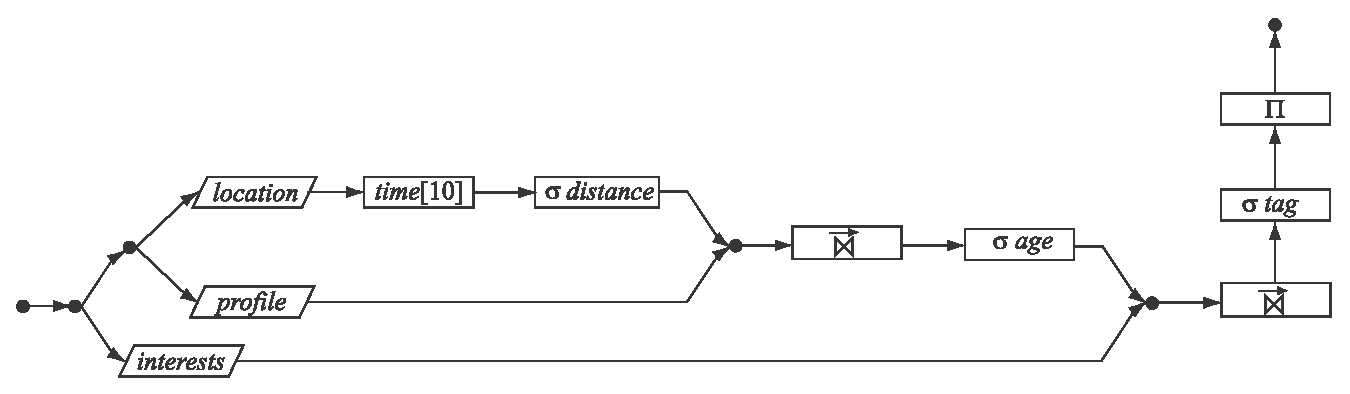
\epsfig{file=Images/FriendFinderQueryWF.eps, scale=0.37}
		\caption{Service-oriented workflow example}
		\label{fig:servCoorExample}
\end{figure}
	
		
\section{Computation services}\label{sec:asasel:computationServices}

Two kinds of computation services form part of our approach: simple computation services and composite computation services specified in the ASASEL language.
	
\textbf{Simple computation services} These involve a single service operation invocation to process data (see Figure \ref{fig:simpleService}). The distance computation service relies on a \texttt{geo-distance} service, which provides the capability to calculate the geographical distance between two points, e.g., by Vincenty's formula.

\textbf{Composite computation services} These process data by multiple operation invocations, possibly from different services, and often also by the manipulation of local data. These tasks are organized in a service coordination specified in the ASASEL language and represented as a workflow, following a model in which we add data items as well as conditional and iteration constructs to our basic parallel and sequential composition workflow model illustrated in Figure \ref{fig:servCoorExample}.
		
Figure \ref{fig:compositeService} depicts a composite computation service, it evaluates the join operator based on the symmetric hash-join algorithm and two instances of a stateful \texttt{hash-index} service. Several interrelated operation invocations on both service instances, as well as reads and updates on local data items, are used to find the tuple matches that form part of the join result.
		
		\begin{figure*}
			\centering
			\begin{tabular}{lr}
				\subfloat[Simple service]{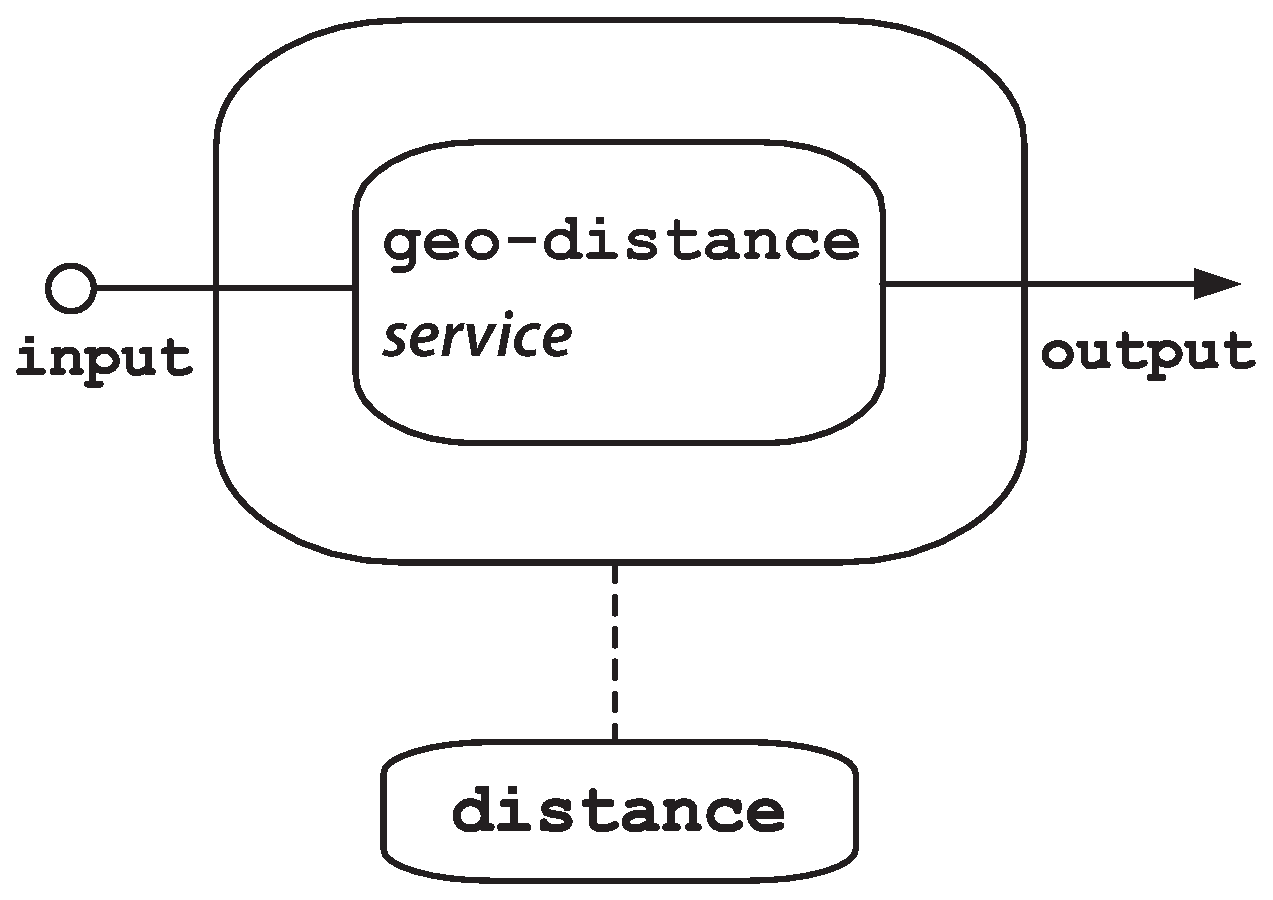
\epsfig{file=Images/Simple.eps, scale=0.2}\label{fig:simpleService}}
				&
				\subfloat[Composite service]{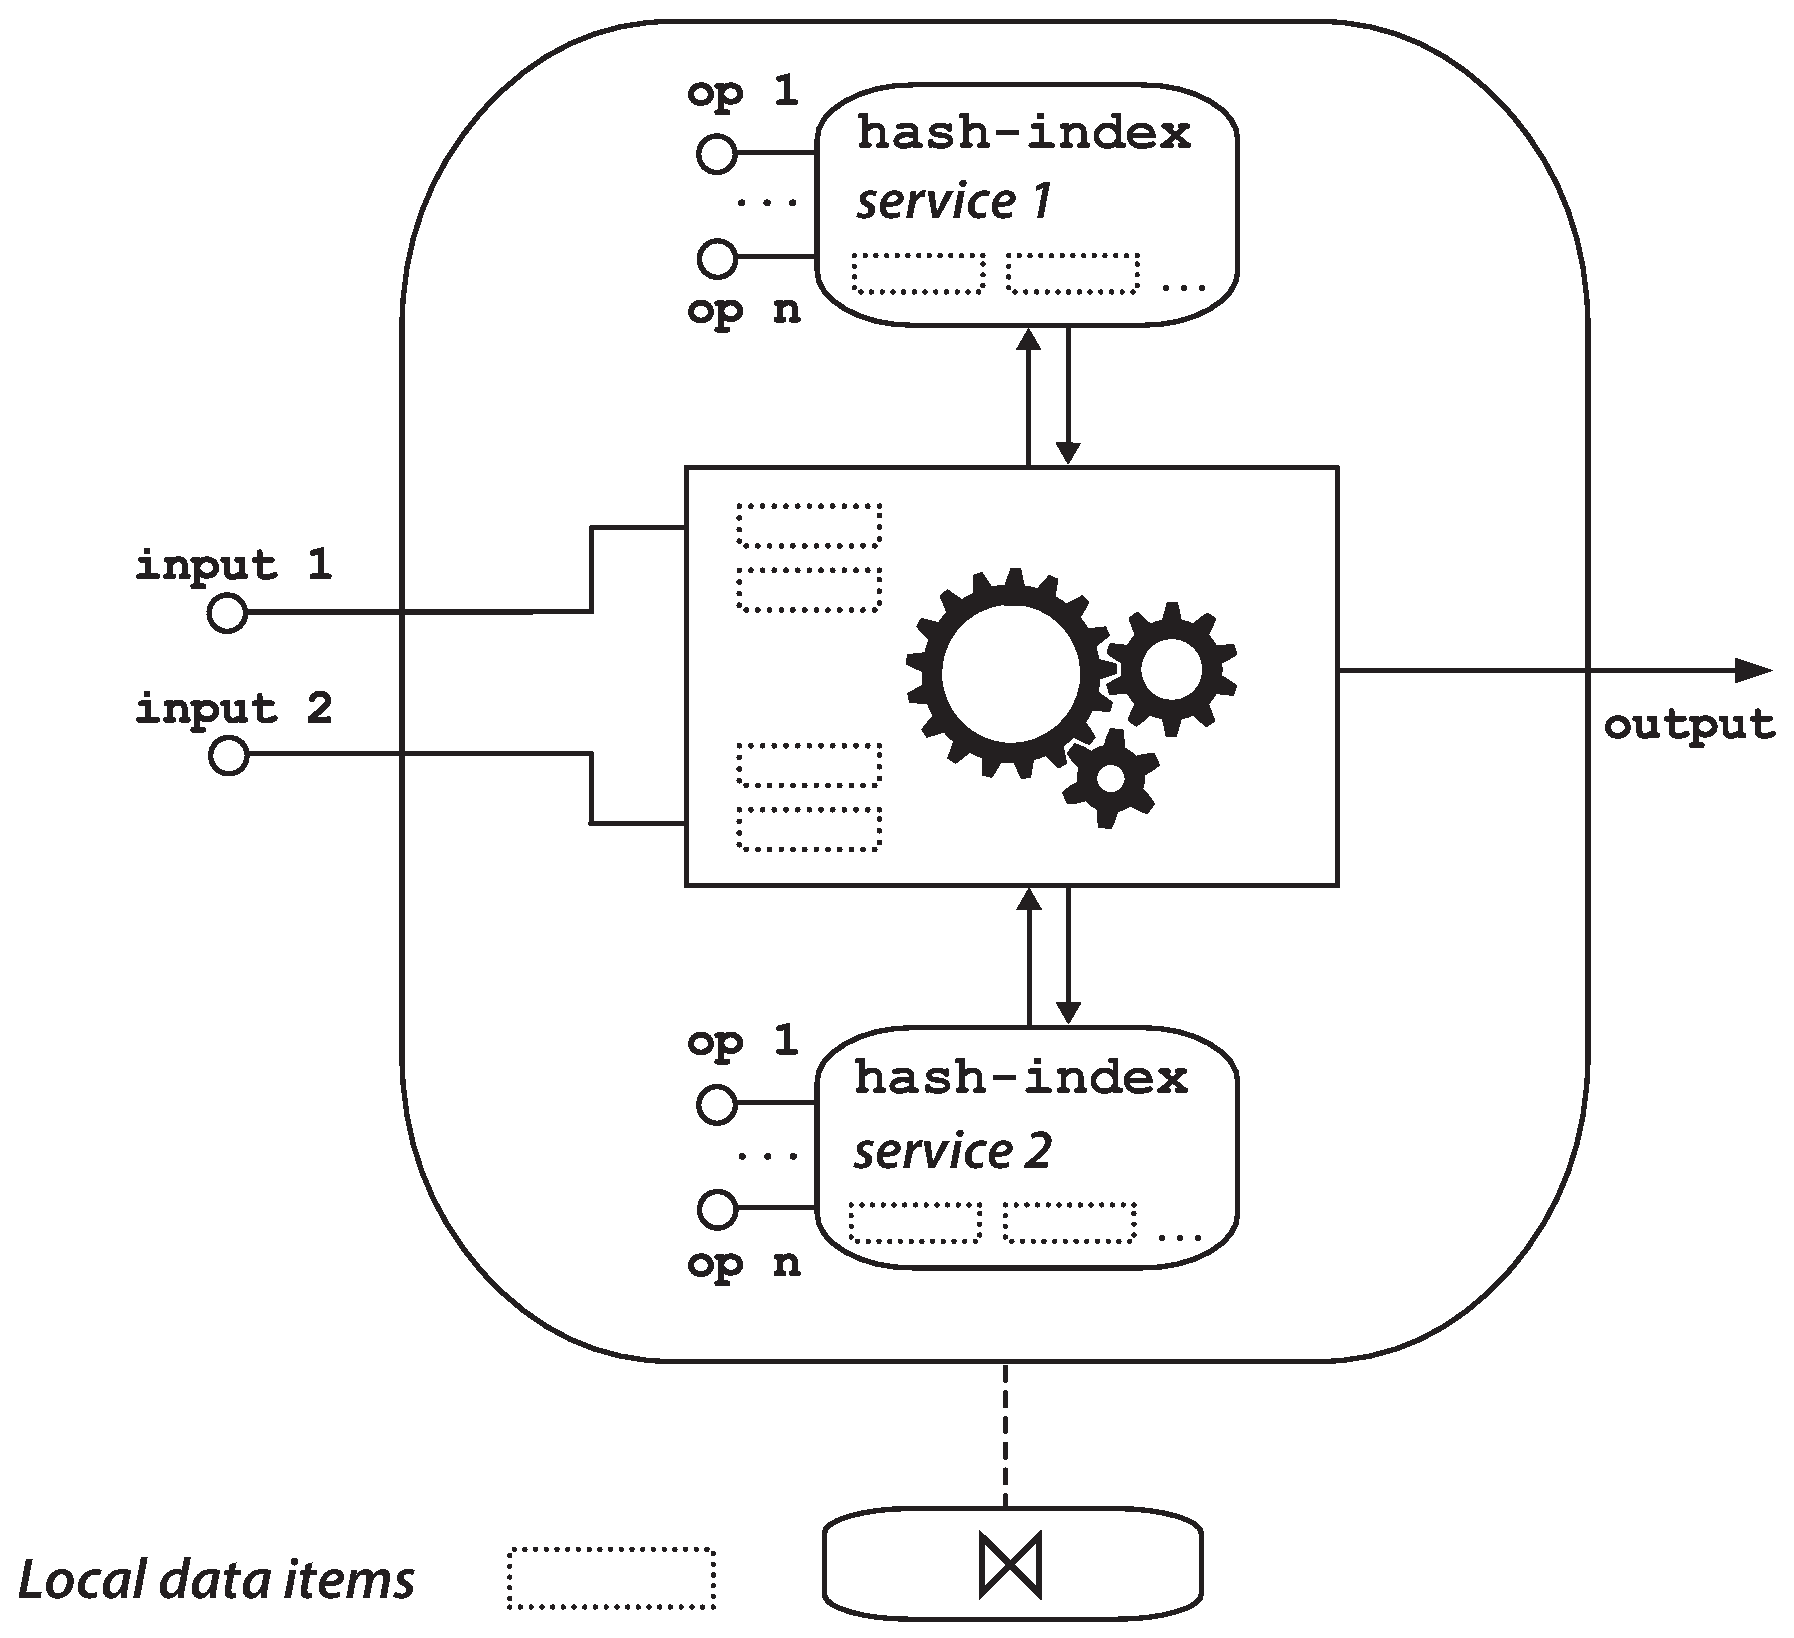
\epsfig{file=Images/Composite.eps, scale=0.2}\label{fig:compositeService}}			
			\end{tabular}
			\caption{Computation services}
			\label{fig:computationServices}
		\end{figure*}
	
\section{Services and Workflow Model}

Next we describe how we model services and their associated workflows, along with the associated quality of service objectives, for our planning-based generation approach.

\subsection{Workflow Quality of Service}

In our framework users express their application needs along their QoS preferences. For instance, consider the application request ``\textit{Where are my friends at this moment?}'' with the QoS preferences ``\textit{Privilege the execution price over the execution time and this in turn on the battery consumption}''.

Services have QoS measures associated to their invocation and thus the overall execution of a workflow has an associated cost that is the aggregation of the QoS measures. For the service-oriented workflows under consideration we assume costs along three dimensions: execution time, execution price, and battery consumption. 

A potentially large finite set of workflows produce the desired results but only a subset from these satisfies the cost requirements of the user. This is a combinatory optimization problem of minimizing the cost of a workflow $W$ that coordinates a subset of activities $A$ through its control-flow. In our workflow generation apporach we limit ourselves to workflows accessing on-demand data only. For example, ``\textit{What are the interests of my friend Joe}'', where only on-demand data are considered.
 
%\begin{equation}
%	\min_{W \subseteq A}\lbrace cost(W): W \text{is a query workflow}\rbrace
%\end{equation}
      
\subsection{Data and computing services}\label{sec:services}

We characterize service APIs with the following structure
			
{\texttt{s\_name:m\_name(B\textsubscript{1}:T\textsubscript{1}?,...,B\textsubscript{m}:T\textsubscript{m}?,F\textsubscript{1}:T'\textsubscript{1}!,...,F\textsubscript{n}:T'\textsubscript{n}!)}}

where the service identified by \texttt{s\_name} has a method named \texttt{m\_name} with \texttt{m} bound parameters, each with an unique name \texttt{B\textsubscript{i}} within the method header and associated with a type \texttt{T\textsubscript{i}}. Analogously there are \texttt{n} free parameters similarly named and typed. Bound and free parameters will be identified by question and exclamation marks, respectively.

From this general notion of service, we distinguish two service specializations as discussed earlier. (1) On-demand data services provide data in a request-response fashion through synchronous data operations. (2) Computing services provide a set of methods to perform operations over data (\eg{}, distance estimation, ordering, correlation).
            
\subsection{Service-oriented workflow} \label{sec:QWModel}
A service-oriented workflow represents a control flow among a set of activities. Each activity is a program that calls a data service method or a computing service method. The control flow is defined by the \textit{sequence} and \textit{parallel} workflow composition operators. 

A service-oriented workflow $W$ is modeled as a directed acyclic graph \textit{W=(V, E, init, finish, A, O)} where:
		\begin{center}
			\footnotesize
			\begin{tabular}{rp{5.5cm}}
				$V$                      & is a set of vertices \\
				$E \subseteq V \times V$ & is a set of edges \\
				$A \subseteq V$          & is a set of activities \\
				$\{init, finish\} \subseteq A$     & are the initial and final activities of $W$\\
				$O \subseteq V$          & is a set of workflow composition operators $\{seq_1,...,seq_m,par_1,...,par_n\}$\\.     
			\end{tabular}   
		\end{center}
               
There are three activity specializations: the \textit{activity} performs a service method invocation and always has a previous and a next activity, the \textit{init} activity has no previous activity and its only goal is to launch the first \textit{activity} of query workflow, the \textit{finish} activity has no next activity and it stops the query workflow execution after the last \textit{activity}.
               
The compositions of activities $E \subseteq V \times V$ are defined by two workflow operators: sequential and parallel composition. A sequential composition $seq$ represents the total order of a pair of activities $a_1,a_2$ such that $e_1=(a_1,a_2)$. It means that the second activity $a_2$ is executed after $a_1$. A parallel composition $par$ represents the partial order of activities $a_1, a_2, a_3, a_4$ such that $e_1=(a_1,a_2)$, $e_2=(a_1,a_3)$, $e_3=(a_2,a_4)$, $e_3=(a_3,a_4)$. It means that $a_2$ and $a_3$ are independent from each other and are executed in parallel after $a_1$ and before $a_4$.
               
\section{Workflow generation} \label{sec:queryWorkflowGen}
      
Workflow generation is the process of enumerating all the valid workflows in order to have a search space for choosing a subset that satisfies the user's preferences. The generation is subject to query workflow constraints for composing activities. We model these constraints as action rules in the language DLV-K\footnote{http://www.dbai.tuwien.ac.at/proj/dlv/k} that allows the sequential or parallel execution of query workflow activities.
         
In DLV-K, planning problems have a set of facts that represent the problem domain named background knowledge. The facts are predicates of static knowledge and are the input of the planning problem. Planning problems are modeled as state machines described by a set of fluents and a set of actions. A fluent is a property of an object in the world and is part of the states of the world \cite{Baral2003}. Fluents may be true, false or unknown. An action is executable if a precondition holds in the current state. Once an action is executed, the fluents and thus the state of the plan are modified. The action rules define the subset of fluents that must be held before the execution of an action (\ie{} pre-conditions) and the subset of fluents to be held after the execution (\ie{} post-conditions). Finally, a goal is a set of fluents that must be reached at the end of plan. A goal is expressed by the conjunction of fluents and by a plan length $l \in \mathds{Z}^{+}$.

The mapping from workflow generation to a planning problem is direct, as shown in Table \ref{tab:mappingQW-PP}. The APIs and the application requirements (operations on data) are modeled as facts of the background knowledge. The execution state of a workflow is modeled as fluents and workflow activities as actions.

	\begin{table}
	   \begin{center}
	      \begin{tabular}{|r|l|}
	         \hline
	         \multicolumn{1}{|c|}{\textbf{Workflow }}& \multicolumn{1}{c|}{\textbf{Planning problem}} \\
	         \hline
	         APIs, operations & Facts (background knowledge) \\
	         \hline
	         Workflow states & Fluents \\
	         \hline
	         Workflow activities & Actions \\
	         \hline
	         Result delivery & Goal: \texttt{finished?(}$l \in \mathds{Z}^{+}$\texttt{)} \\
	         \hline
	      \end{tabular}
	   \end{center} 
	   \caption{Mapping to a planning problem for a workflow}
	   \label{tab:mappingQW-PP}
	\end{table}

Next we show, through a simple example, how we represent the background knowledge for workflow generation. Afterwards, we show how the workflow state and activities are expressed in DLV-K.
         
\subsection{Background knowledge} \label{subsec:kb}
The background knowledge is the input for workflow generation and it is represented by a set of facts. The facts are two-folded in (1) service interface representation and (2) operations representation.
               
\textbf{Service interface} Consider the following service methods:

{\footnotesize\texttt{p:profl(str:nickname?,int:age!,str:sex!,str:email!)}}

This method provides the user profile formed by \texttt{age, sex} and \texttt{email} of a given user with a \texttt{nickname}.

{\footnotesize\texttt{i:interests(str:nickname?,str:tag!,real:score!)}}

This method provides the interests of a given user identified by a \texttt{nickname}. An interest is represented by a \texttt{tag} and has a \texttt{score} that quantifies the interest over the tag.

The service interface and its methods are described by the facts \texttt{service_interface/1} and the \texttt{method/2} respectively. We distinguish between bound and free parameters with the facts \texttt{bound_p/4} and \texttt{free_p/4}. The normal form of a parameter is stated by \texttt{parameter/4} and this rule guarantees that the parameter name is unique in the context of the service method.

%\lstinputlisting[lastline=15, fontadjust=true, label=list:service-interfaces,caption={Service interfaces}]{code/service-interfaces-FF.kb}

\lstinputlisting[lastline=15, fontadjust=true, label=list:service-interfaces]{code/service-interfaces-FF.kb}
            
\textbf{Operations} Now consider the application requirement ``\textit{What are the interests of my friend Joe}'' that is represented by the operation facts:

%\lstinputlisting[fontadjust=true, label=list:hybridQuery, caption={Hybrid query in facts}]{code/query-FF1.kb}

\lstinputlisting[fontadjust=true, label=list:hybridQuery]{code/query-FF1.kb}

This requirement expresses the need of data over the methods \texttt{p:profl} and \texttt{i:interests} methods, the nickname of the profile is filtered and correlated with the nickname of interests. Finally, the parameters nickname, score and tag are projected. Observe that the selection over the nickname attribute is indicated only in intention because the equality operators are not significant for the workflow generation.

\subsection{Workflow activities}
Workflow activities are represented as actions in DLV-K. In general, the activities are predicates that hold if their facts from background knowledge are true. There are also activities that are independent from facts.
         
\textbf{init and finish} These activities have the special purpose to \texttt{init} and \texttt{finish} the workflow execution accordingly with our model in subsection \ref{sec:QWModel}. Thus the semantics is not associated with the application and there is no dependency with the background knowledge.

\textbf{on-demand} This activity establishes a connection with a data service method and requires a method of a service and the expressed need of the user to be fulfilled.

%\lstinputlisting[firstline=23, lastline=23, fontadjust=false, label=list:qw-on-demand, caption={on-demand activity}]{code/aesop.plan}

\lstinputlisting[firstline=23, lastline=23, fontadjust=false, label=list:qw-on-demand]{code/aesop.plan}

\textbf{bind_selection}
This activity invokes and retrieves data from a service method. The invocation is done by a given bound parameter valid in the service interface definition. The workflow must express which data are required from this service method in respect to a selected bound parameter.

%\lstinputlisting[firstline=26, lastline=27, fontadjust=false, label=list:qw-bind-selection, caption={bind-selection activity}]{code/aesop.plan}

\lstinputlisting[firstline=26, lastline=27, fontadjust=false, label=list:qw-bind-selection]{code/aesop.plan}

\textbf{bind_join} The required correlation in the workflow is performed by this activity. Correlation is binary between data from two service methods on a parameter from each one. The parameter from the outer method must be bound. This activity is analogous to \texttt{bind_selection} but this one takes the value of a bound parameter from the output of another method (\ie{} the inner method).
                     
%\lstinputlisting[firstline=30, lastline=35, fontadjust=false, label=list:qw-bind-join, caption={bind-join activity}]{code/aesop.plan}

\lstinputlisting[firstline=30, lastline=35, fontadjust=false, label=list:qw-bind-join]{code/aesop.plan}
                     
\textbf{select} The select activity performs the filtering over a parameter of a required service method.
            
%\lstinputlisting[firstline=39, lastline=42, fontadjust=false, label=list:qw-select, caption={select activity}]{code/aesop.plan}

\lstinputlisting[firstline=39, lastline=42, fontadjust=false, label=list:qw-select]{code/aesop.plan}
                     
\textbf{project} This activity projects a parameter of a service method.
                     
%\lstinputlisting[firstline=44, lastline=44, fontadjust=false, label=list:qw-project, caption={project activity}]{code/aesop.plan}

\lstinputlisting[firstline=44, lastline=44, fontadjust=false, label=list:qw-project]{code/aesop.plan}
				   
The semantics of activities described above is completed with constraints that define their pre-conditions and post-conditions.
				
\subsection{Workflow constraints} These constraints define the conditions associated to the execution of activities. A condition is a state of knowledge modifiable by the execution of the activities. Conditions also define when the activities can be executed. Hence, we talk about pre-conditions and post-conditions of activities. A state is composed by a set of fluents that occur during the execution of activities. The rules that define when a fluent occurs can be static or dynamic. Static rules are those that occur given the truth-value of a subset of fluents, and dynamic rules occur given the truth-value of a subset of fluents and after the execution of an activity.
               
Below we present the constraints that describe how the activities can be performed and how a query plan should be constructed.
               
\textbf{init and finish} The first executable activity in a query workflow is \textbf{init}. This activity has no previous activity, thus its pre-condition is that the query workflow is not \texttt{initiated} and produces a new state \texttt{initiated}. The last activity is \texttt{finish} and there is no other activity executed after this one. The pre-condition to execute \texttt{finish} is that there is not evidence that the query workflow is \texttt{finished} and the data is already \texttt{delivered} (See \texttt{output} activity below for details about \texttt{delivered}). The post-condition of \texttt{finish} is \texttt{finished} and this is always the goal for the generation.
                            
%\lstinputlisting[firstline=49, lastline=52, fontadjust=false, label=list:init-activity, caption={\texttt{init} and \texttt{finish} activities}]{code/aesop.plan}

\lstinputlisting[firstline=49, lastline=52, fontadjust=false, label=list:init-activity]{code/aesop.plan}
                   
\textbf{on-demand} Once initiated the plan, the data services must be \texttt{connected(DS)}. This fluent is produced by the execution of \texttt{on_demand(DS)} activity. 

%\lstinputlisting[firstline=55, lastline=56, fontadjust=false, label=list:on-demand-activity, caption={on-demand activity}]{code/aesop.plan}

\lstinputlisting[firstline=55, lastline=56, fontadjust=false, label=list:on-demand-activity]{code/aesop.plan}

During the execution, all data services must be connected. Therefore, there is a fluent \texttt{all_connected} that is false if there is not evidence that a data service is connected. Otherwise, it is true.

%\lstinputlisting[firstline=58, lastline=59, fontadjust=false, label=list:all-connected-fluent, caption={all\_connected fluent}]{code/aesop.plan}

\lstinputlisting[firstline=58, lastline=59, fontadjust=false, label=list:all-connected-fluent]{code/aesop.plan}
     
\textbf{bind_selection} One of the activities that implements data retrieval is bind selection. It is only executable if there is not evidence that the data service \texttt{DS} has already been retrieved and if there is a connection with \texttt{DS}. Once the bind selection is executed, the fluent \texttt{retrieved(DS)} is true. \texttt{retrieved(DS)} is an inertial fluent, thus the re-execution is not possible. 
      
%\lstinputlisting[firstline=61, lastline=63, fontadjust=false, label=list:bind-selection-activity, caption={bind\_ selection activity}]{code/aesop.plan}

\lstinputlisting[firstline=61, lastline=63, fontadjust=false, label=list:bind-selection-activity]{code/aesop.plan}

\textbf{selection} The filtering of data is done by the \texttt{selection} activity. It is executable if there is not evidence that the parameter \texttt{P} of \texttt{DS} has already been selected. There is also need that the data from \texttt{DS} has been retrieved and obviously the selection \texttt{select_(DS,P)} must be part of the workflow. The execution of the selection makes the fluent true \texttt{selected(DS,P)} and it is inertial, so the re-execution of the selection \texttt{select(DS,P)} is not possible.

%\lstinputlisting[firstline=74, lastline=76, fontadjust=false, label=list:select-activity, caption={select activity}]{code/aesop.plan}

\lstinputlisting[firstline=74, lastline=76, fontadjust=false, label=list:select-activity]{code/aesop.plan}

In order to be aware of the state of selection over all the required parameters of a method \texttt{DS}, the all_selected_from(DSOName) becomes true if there is no other parameter pending to be selected.

%\lstinputlisting[firstline=77, lastline=78, fontadjust=false, label=list:all-selected-from, caption={all\_select\_from fluent}]{code/aesop.plan}

\lstinputlisting[firstline=77, lastline=78, fontadjust=false, label=list:all-selected-from]{code/aesop.plan}

Analogously, all parameters from all data services must be selected when they are required. Therefore, there is the fluent \texttt{all\_selected}. This fluent is true if there is no other method \texttt{DS} pending to be selected.

%\lstinputlisting[firstline=80, lastline=82, fontadjust=false, label=list:all-selected, caption={all\_select fluent}]{code/aesop.plan}

\lstinputlisting[firstline=80, lastline=82, fontadjust=false, label=list:all-selected]{code/aesop.plan}

\textbf{projection} This activity is executable if there is not evidence that the parameter \texttt{P} of \texttt{DSOName} has been projected. There is also need that the data from \texttt{DSOName} be retrieved. The execution of projection makes the fluent \texttt{projected(DSOName,P)} true and it is inertial, thus the re-execution of the projection is not possible.
               
%\lstinputlisting[firstline=84, lastline=85, fontadjust=false, label=list:project, caption={project activity}]{code/aesop.plan}

\lstinputlisting[firstline=84, lastline=85, fontadjust=false, label=list:project]{code/aesop.plan}

The projected fluent is true once the action \texttt{project(DS,P)} is done. During the query workflow execution, all the required parameters must be projected. For \texttt{DS} grain the fluent \texttt{all\_projected\_from(DS)} is true if there is no other parameter from \texttt{DS} pending to be projected. For the entire query, the fluent \texttt{all\_projected} is true if there is no other \texttt{DS} pending to be projected.
                
%\lstinputlisting[firstline=88, lastline=92, fontadjust=false, label=list:all-projected-from, caption={all\_projected\_from fluent}]{code/aesop.plan}

\lstinputlisting[firstline=88, lastline=92, fontadjust=false, label=list:all-projected-from]{code/aesop.plan}
                    
\textbf{output} Once the operations are processed, data must be delivered by the activity \texttt{output}. In order to model this precondition, the fluent \texttt{query\_processed} is true if all the other possible activities have been processed. Otherwise, the fluent is \texttt{-query\_processed}.

%\lstinputlisting[firstline=95, lastline=99, fontadjust=false, label=list:query-processed, caption={query\_processed fluent}]{code/aesop.plan}

\lstinputlisting[firstline=95, lastline=99, fontadjust=false, label=list:query-processed]{code/aesop.plan}

Once the query is processed, the \texttt{output} activity delivers the result and the fluent \texttt{delivered} becomes true.

%\lstinputlisting[firstline=101, lastline=102, fontadjust=false, label=list:output, caption={output fluent}]{code/aesop.plan}

\lstinputlisting[firstline=101, lastline=102, fontadjust=false, label=list:output]{code/aesop.plan}

\section{Experiments} \label{sec:experiments} We performed experiments with the various sets of operation instances described below. The objective of the experiments is to measure the size of the search space of query workflows given a fixed number of activities and a goal to define the length of the workflow.

\subsection{Configuration} In order to test the performance of workflow generation, we have defined four test cases. All are based on the example of subsection \ref{subsec:kb}. In order to make the generation more complex we add two data operations. The resulting workflows are configured as follows:

	\begin{table*}         	
		\begin{center}
		{\footnotesize
			\begin{tabular}{|c|c|c|l|c|}
				\hline
					  & \multicolumn{2}{c|}{Data operator} & \multirow{3}{*}{Description} & \multirow{3}{*}{\# activities}\\
				\cline{1-3}
				Query & \tiny{select_(p,age)}&\tiny{join_(p,nickname,i.nickname)}& &\\
				\hline
				[Q1]  & \tickNo  & \tickNo & no additional operators& 11 \\
				\hline
				[Q2] & \tickYes & \tickNo & +unary data operator  & 12 \\
				\hline
				[Q3] & \tickNo  & \tickYes & +binary operator  & 13\\
				\hline
				[Q4] & \tickYes & \tickYes & +both unary and binary operator& 14 \\
				\hline
			\end{tabular}
		}
		\end{center}\caption{Workflow configuration} \label{tab:queryConf}
	\end{table*}
	

Another dimension for the test is the max length of plans. The generated plans depend on a required plan length. In DLV-K, one must specifies the desired length that determines the size of the search space of query workflows and thus the required time for the generation.
      
In the tests we used lengths from 6 to 14, and we will measure (1)the length of the generated plans, (2)the size of the search space, and (3) the execution time of the generation.
         
\subsection{Results}

The data retrieved from the experiments show (1) the behavior of the search space growth during the generation and (2) the time required for generating all the search space.  
		
Each workflow requires a fixed number of activities accordingly with the number of data operators required to process its result. Given that size of query plans are subject to the length $l$, there are workflows that require a largest $l$ than others.
For example, $Q1$ with $11$ activities, requires at least an $l=7$ to get workflows with the must possible parallel compositions, and at most $l=11$ to get completely sequential compositions. For space reasons we invite the reader to visit the URLs http://goo.gl/XKZuL and http://goo.gl/z4iu3 to appreciate examples of query workflows of 7-length and 11-length respectively.
\tabsize{tab:tablesize}{Search space growth respect to the plan length}
The growth of search space is shown in Table \ref{tab:tablesize} and, as was expected, the size of search space tends to be stable once the maximum length is reached. For example, $Q1$ reach the maximum length with $l=11$. This is analogous for $Q2$, $Q3$, and $Q4$. Nevertheless the size of search space for each one is considerably bigger than the others less complex. It can be noted that the search spaces have an exponential growth until the max length.
		
%		\begin{figure*}
%           \begin{center}
%               \begin{tabular}{ccc}
%
%			        \subfloat[Search space growth respect to the plan length]{\epsfig{file=Images/size.eps, scale=0.45}\label{subfig:graphsize}} & &
%			        %\subfigure[Complex]{\epsfig{figure=Images/WFComplexActivity.eps,scale=0.6}\label{subfig.complexActivity}} &
%			        \subfloat[Behavior of query workflow generation during the time]{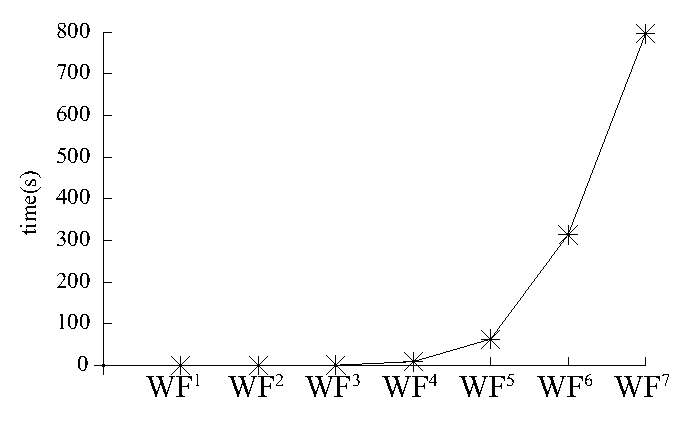
\epsfig{file=Images/time.eps, scale=0.45}\label{subfig:graphtime}}
%                \end{tabular}
%            \end{center}
%        \end{figure*}
        
Besides the size of search space, the time for processing the workflow generation is also exponential  and it is not feasible to generate completely the search space in the context of query optimization. Thus, this enumeration must be done implicitly in order to avoid the combinatorial explosion.
		
\section{System Implementation} \label{sec:asasel:demo}
	
The ASASEL system was developed on the Java platform. Workflows are entered textually via a GUI illustrated in Figure \ref{fig:asaselGUI}. For a given ASASEL service coordination, the GUI (relying on the JGraph\footnote{http://www.jgraph.com/} library) provides the user a workflow visualization. Data services are represented in yellow whereas computation services are represented in blue, both with their corresponding labels.

The enactment of a workflow is enabled by two main components. First, a scheduler determines which service is executed at a given time according to a predefined policy. Second, composite services are executed by an interpreter that implements the full ASASEL language. Computation service workflows can also be visualized through the GUI, as shown at the right part of the screenshot in Figure \ref{fig:asaselGUI}. The interpreter was developed using the ANTLR\footnote{http://www.antlr.org/} parser generator.
	
During the execution of a workflow, data flows from the data services to several computation services via queues, as determined by the ASASEL specification. Computation services can be specified to output data in textual form in the GUI or to transmit it to another application. For instance, in our example application we output as a result data stream that denotes the tuples that are added and the tuples that are removed from the result dataset.
	
We developed a set of basic computation services that are used to build the operations for our example application. These services run on a Tomcat container supported by the JAX-WS reference implementation \footnote{https://jax-ws.dev.java.net/}, which enables to create stateful services.
	
Additionally, we implemented two test scenarios and their corresponding data services to use with our computation services. The first one is the location-based application introduced in Section \ref{sec:asasel:example}. The second scenario is an adaptation of the NEXMark benchmark\footnote{http://datalab.cs.pdx.edu/niagara/NEXMark/} for XML stream query processing which we employed to obtain performance measurements. In brief, the measurements indicated a tolerable overhead for the use of services, which we consider outweighed by the advantages.
	
	%\begin{figure*}
	%	\centering
	%	\epsfig{file=Images/ASASEL.eps, scale=0.37}
	%	\caption{}
	%	\label{fig:asaselGUI}
	%\end{figure*}
	
	\begin{figure}
   \begin{center}
      \scalebox{0.675}{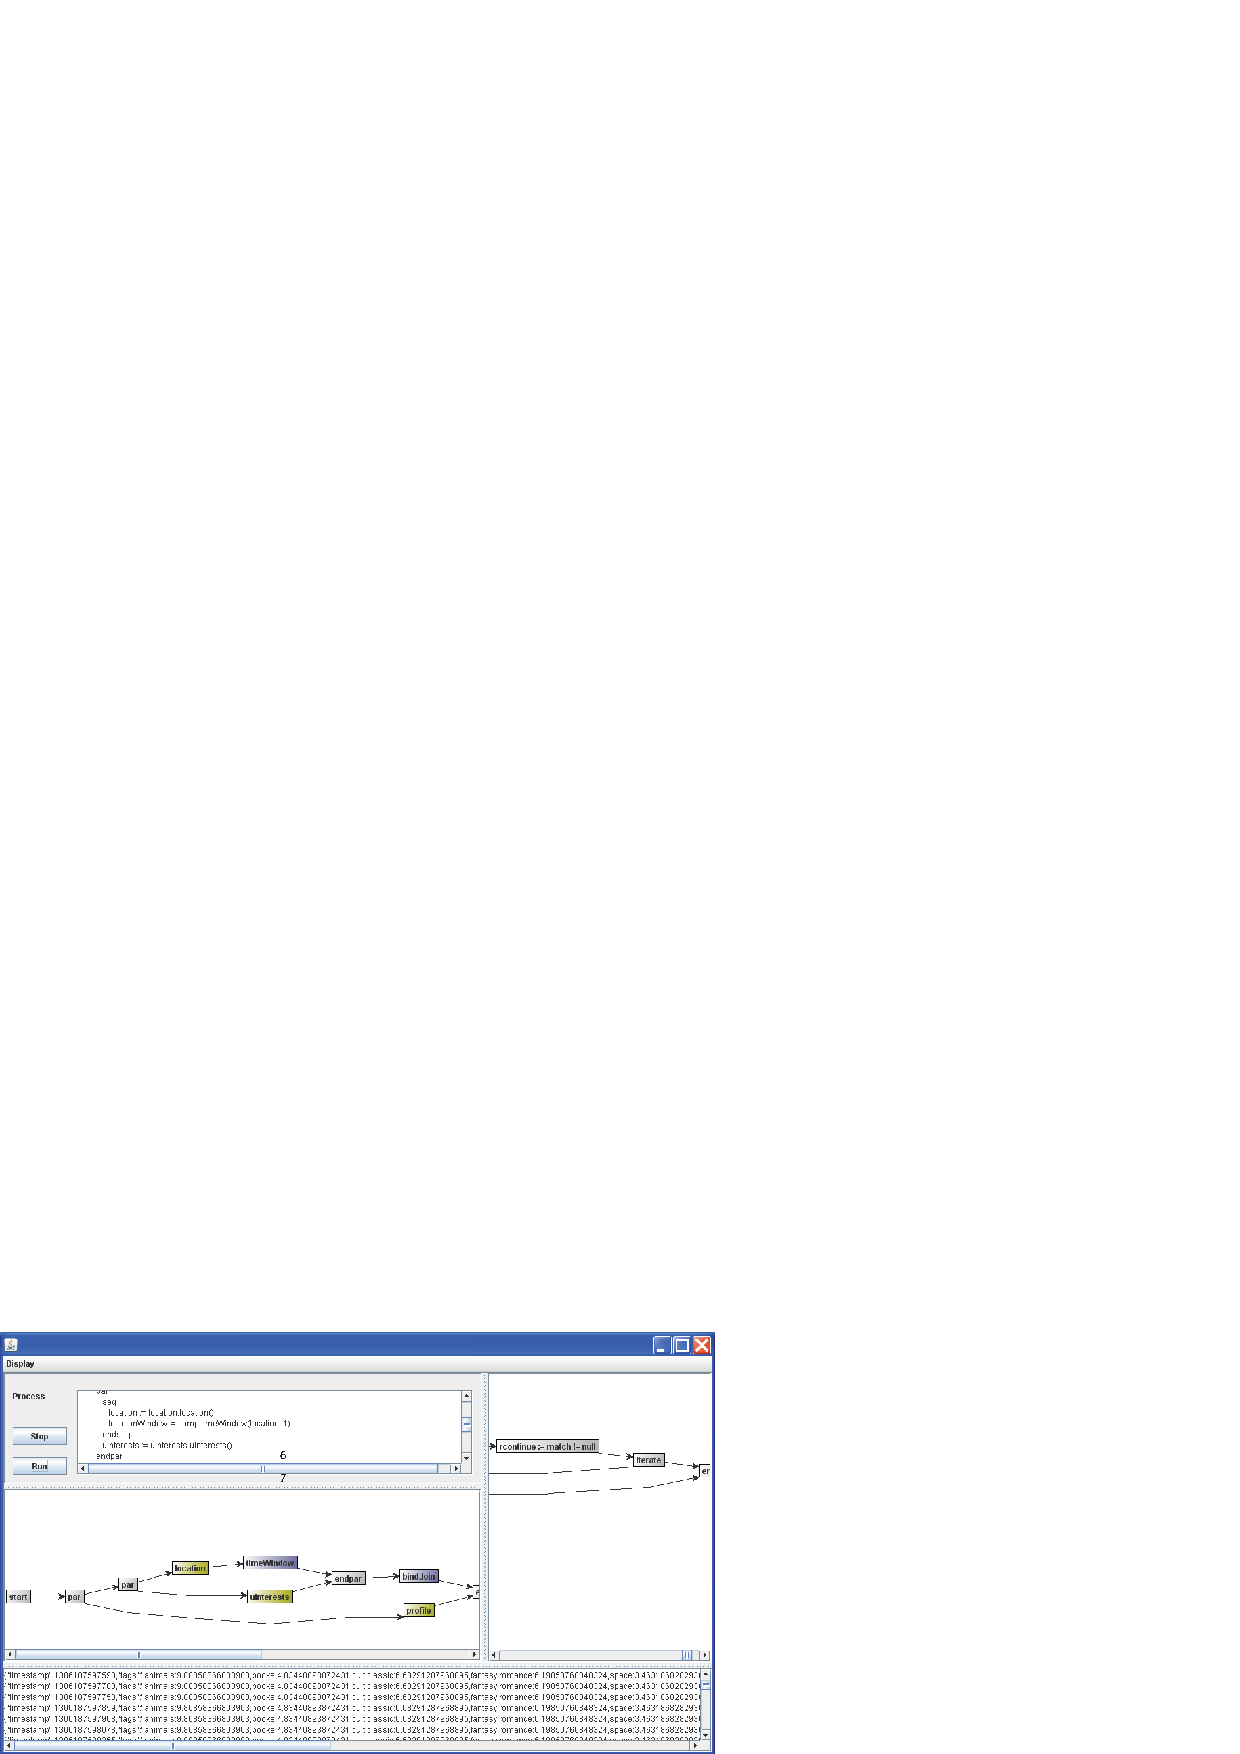
\includegraphics[natwidth=12.31cm,natheight=7.16cm]{Images/asaselgui.pdf}}
   \end{center}
   \caption{Caption of the ASASEL GUI}
   \label{fig:asaselGUI}
\end{figure}
	
\section{Related work} \label{sec:relatedwork}

The optimization of workflows involving data services must tackle challenges such as autonomy, non-durability of data, absence of fine grain data statistics, etc. For instance, the evaluation of queries over Web services presented in \cite{Srivastava2006} proposes an optimization approach by ordering the service calls in a pipelined fashion and by tunning the size of data. However, the control over data size (i.e. data chunks) and selectivity statistics is a strong assumption because of the autonomy of services and the absence of data statistics in many real scenarios.

Another aspect to consider during the optimization is the selection of the service instances, which represents a factor for the service coordination cost. In \cite{Claro2005,Wada2008} the optimal selection of services with a multidimensional cost is proposed for optimizing the complete service coordination. This selection is done by solving a multi-objective assignation problem for a set of abstract services. However, the possibility to modify the order of service invocations is not considered and this is a key issue in service-oriented workflow optimization.

\section{Conclusions and future work} \label{sec:conclusion}

In this paper we focused on the generation of the search space of data-centric workflows in service-oriented environments. We proposed a set of constraints modeled in an action language, specifically DLV-K, in order to characterize the construction of workflows with sequential and parallel compositions.This work is envisaged to be a foundation for incorporating a full cost model, leading to the selection of the most suitable workflow w.r.t. user's preferences. This is crucial because in the absence of constraints the search space is in the order of $n!$ permutations in the number of activities required for obtaining the result.

%}
%	In this paper we presented the constraints for generating query workflows that model the plans of hybrid queries.
%	The constraints represent the semantics of query workflow activities that is that implement data operators for evaluating a hybrid query.
%	We used the action language DLV-K for modeling the planing problem of query workflow generation in order to get a first (and naive) search space generation towards the optimization of hybrid queries.
%	The results show that time complexity for query workflow generation is exponential. 
%      
%	The constraints must be extended in order to consider the continuous data operators for completely modeling hybrid queries.
%	These constraints can be taken to model a more sophisticated query workflow generation.
%	This implies the abstraction of data operators types and their associated constraints in a general form. 
%
%	Theoretically, query workflow generation can be modeled mathematically by taking the constraints presented here and modeling an objective function.
%	Additionally, the equivalence and coherence of query workflows must be proved.


	
%
% ---- Bibliography ----
%
%\bibliographystyle{alpha}
\bibliographystyle{abbrv}
\bibliography{library/library}

\end{document}
